\section{Application: Simplification of quadratic forms}

In this section, we will explore an application of the diagonalization
of symmetric matrices, namely, the simplification of quadratic forms.
Quadratic forms are special kinds of functions that arise, for
example, in calculus when we approximate some quantity up to terms of
second order.

\begin{definition}{Quadratic form}{quadratic-form}
  A \textbf{quadratic form}%
  \index{quadratic form} is a polynomial in $n$ variables in which
  each term is of degree 2. For example, the following is a quadratic
  form in $3$ variables:
  \begin{equation*}
    f(x,y,z) = 3x^2 + 3y^2 + 2xy - 4xz + 4yz.
  \end{equation*}
  More generally, a quadratic form is a function of the form
  \begin{equation*}
    f(x_1,\ldots,x_n) = q_1\,x_1^2 + \ldots + q_n\,x_n^2 + q_{12}\,x_1x_2 +
    \ldots + q_{ij}\,x_ix_j + \ldots + q_{n-1,n}\,x_{n-1}x_n.
  \end{equation*}
  The numbers $q_1,\ldots,q_n,q_{12},\ldots,q_{n-1,n}$, which may be
  positive, negative, or zero, are called the \textbf{coefficients}%
  \index{coefficient!of a quadratic form}%
  \index{quadratic form!coefficient} of the quadratic form.
\end{definition}

\begin{example}{Quadratic forms}{quadratic-form}
  Which of the following are quadratic forms?
  \begin{enumialphparenastyle}
    \begin{enumerate}
    \item $f(x,y,z) = 2xy + 3xz - 5yz$.
    \item $g(x,y,z) = x^2 + 2xy + y^2 + 3$.
    \item $h(x,y,z) = (x+y)^2 - z^2$.
    \end{enumerate}
  \end{enumialphparenastyle}
\end{example}

\begin{solution}
  The function $f$ is a quadratic form. The function $g$ is not a
  quadratic form, because the constant term, $+3$, is not of degree
  2. It should be either a coefficient times the square of a variable,
  or a coefficient times the product of two variables. The function
  $h$ is a quadratic form. We can simplify it to $h(x,y,z) = x^2 + 2xy
  + y^2 - z^2$.
\end{solution}

\begin{definition}{Matrix form of a quadratic form}{quadratic-form-matrix}
  Let $A$ be a symmetric $n\times n$-matrix, and let
  $\vect{v} = \mat{x_1,\ldots,x_n}^T$.  Then
  \begin{equation*}
    f(x_1,\ldots,x_n) = \vect{v}^T A\vect{v}
  \end{equation*}
  is a quadratic form in $n$ variables. Conversely, every quadratic
  form in $n$ variables can be uniquely written in this way. We call
  this the \textbf{matrix form} of the quadratic form%
  \index{quadratic form!matrix form}%
  \index{matrix form of quadratic form}.
\end{definition}

\begin{example}{Matrix form of a quadratic form}{quadratic-form-matrix}
  Find the coefficients of the quadratic form $f(x,y,z) = \vect{v}^T
  A\vect{v}$, where
  \begin{equation*}
    A = \begin{mymatrix}{rrr}
      1 &  2 &  4 \\
      2 &  0 & -1 \\
      4 & -1 & -2 \\
    \end{mymatrix}.
  \end{equation*}
\end{example}

\begin{solution}
  We have
  \begin{equation*}
    f(x,y,z)
    ~=~
    \begin{mymatrix}{ccc} x & y & z \end{mymatrix}
    \begin{mymatrix}{rrr}
      1 &  2 &  4 \\
      2 &  0 & -1 \\
      4 & -1 & -2 \\
    \end{mymatrix}
    \begin{mymatrix}{c} x \\ y \\ z \end{mymatrix}
    ~=~ x^2 - 2z^2 + 4xy + 8xz - 2yz.
  \end{equation*}
  Note that there is a term $2xy$ and a term $2yx$, which together
  yield $4xy$. Similarly the term $4xz$ and $4zx$ are combined into
  $8xz$, and the terms $-yz$ and $-zy$ are combined into $-2yz$.
\end{solution}

\begin{example}{Matrix form of a quadratic form}{quadratic-form-matrix2}
  Write the quadratic form
  \begin{equation*}
    f(x,y,z) = 5x^2 - y^2 + z^2 + 2xy - 4xz + 3yz
  \end{equation*}
  in matrix form.
\end{example}

\begin{solution}
  We can write this as
  \begin{equation*}
    f(x,y,z)
    ~=~
    \begin{mymatrix}{ccc} x & y & z \end{mymatrix}
    \begin{mymatrix}{rrr}
      5  &   1 &  -2 \\
      1  &  -1 & 1.5 \\
      -2 & 1.5 &   1 \\
    \end{mymatrix}
    \begin{mymatrix}{c} x \\ y \\ z \end{mymatrix}.
  \end{equation*}
  Note: since the matrix $A$ must be symmetric, we have no choice but
  to split the term $2xy$ evenly into $1xy$ and $1yx$. This explains
  why the $(1,2)$- and $(2,1)$-entries of the matrix are $1$. Also,
  $-4xz$ has been split into $-2xz$ and $-2zx$, and $3yz$ has been
  split into $1.5yz$ and $1.5zy$. In general, the matrix of the
  quadratic form
  \begin{equation*}
    f(x,y,z) = ax^2 + by^2 + cz^2 + dxy + exz + fyz
  \end{equation*}
  is
  \begin{equation*}
    \def\arraystretch{1.3}
    A = \begin{mymatrix}{rrr}
      a & \frac{d}{2} & \frac{e}{2} \\
      \frac{d}{2} & b & \frac{f}{2} \\
      \frac{e}{2} & \frac{f}{2} & c \\
    \end{mymatrix}.
  \end{equation*}
\end{solution}

We will now turn to the question of how to simplify quadratic
forms. The primary tool we have for doing so is a \textbf{change of
  variables}%
\index{change of variables!for a quadratic form}%
\index{quadratic form!change of variables}. This means replacing the
variables $x_1,\ldots,x_n$ by new variables $y_1,\ldots,y_n$ that are
linear combinations of $x_1,\ldots,x_n$.

\begin{example}{Change of variables}{quadratic-form-change-of-variables}
  Apply the change of variables
  \begin{eqnarray*}
    x &=& u \\
    y &=& v-w \\
    z &=& w
  \end{eqnarray*}
  to the quadratic form
  \begin{equation*}
    3x^2 + y^2 + 2xy + 2xz + 2yz
  \end{equation*}
\end{example}

\begin{solution}
  We have
  \begin{equation*}
    \begin{array}{l}
      3x^2 + y^2 + 2xy + 2xz + 2yz \\
      =~~ 3u^2 + (v-w)^2 + 2u(v-w) + 2uw + 2(v-w)w \\
      =~~ 3u^2 + v^2 - w^2 + 2uv.
    \end{array}
  \end{equation*}
\end{solution}

The simplest kind of quadratic form is one that involves only squared
variables, and no products of two different variables. We call such
quadratic forms \textbf{diagonal}.

\begin{definition}{Diagonal quadratic form}{diagonal-quadratic-form}
  A quadratic form is \textbf{diagonal}%
  \index{diagonal quadratic form}%
  \index{quadratic form!diagonal} if it is of the form
  \begin{equation*}
    f(x_1,\ldots,x_n) = q_1\,x_1^2 + \ldots + q_n\,x_n^2.
  \end{equation*}
\end{definition}

\begin{proposition}{Diagonalization of quadratic forms}{quadratic-form-diagonalize}
  Every quadratic form can be made diagonal by a change of variables.
\end{proposition}

\begin{proof}
  We first write the quadratic form in matrix form, i.e.,
  \begin{equation*}
    f(x_1,\ldots,x_n) = \vect{v}^T A \vect{v},
  \end{equation*}
  where $A$ is a symmetric matrix and
  $\vect{v}=\mat{x_1,\ldots,x_n}^T$. By
  Theorem~\ref{thm:diagonalization-symmetric}, $A$ is orthogonally
  diagonalizable. So let $P$ be an orthogonal matrix such that
  \begin{equation*}
    P^{-1}AP
    ~=~ P^TAP
    ~=~ D
    ~=~ \begin{mymatrix}{ccc}
      \eigenvar_{1} & \cdots & 0      \\
      \vdots & \ddots & \vdots \\
      0      & \cdots & \eigenvar_{nn} \\
    \end{mymatrix}
  \end{equation*}
  is diagonal. Let $\vect{w}=\mat{y_1,\ldots,y_n}^T$ be a new set of
  variables such that $\vect{v} = P \vect{w}$.  Then
  \begin{equation*}
    \vect{v}^T A \vect{v}
    ~=~ \vect{w}^T P^TAP \vect{w}
    ~=~ \vect{w}^T D \vect{w}
    ~=~ \eigenvar_{1}y_1^2 + \ldots + \eigenvar_{n}y_n^2.
  \end{equation*}
  So the quadratic form is diagonal in the variables $y_1,\ldots,y_n$.
\end{proof}

\begin{example}{Diagonalization of quadratic forms}{quadratic-form-diagonalize}
  Consider the quadratic form
  \begin{equation*}
    f(x,y) = 3x^2 + 4xy + 6y^2.
  \end{equation*}
  Perform a change of variables so that the quadratic form becomes diagonal.
\end{example}

\begin{solution}
  We first write $f(x,y)$ in matrix form:
  \begin{equation*}
    f(x,y)
    = \begin{mymatrix}{cc} x & y \end{mymatrix}
    \begin{mymatrix}{rr} 3 & 2 \\ 2 & 6 \end{mymatrix}
    \begin{mymatrix}{c} x \\ y \end{mymatrix}.
  \end{equation*}
  Next, we orthogonally diagonalize the matrix
  $A = \begin{mymatrix}{rr} 3 & 2 \\ 2 & 6 \end{mymatrix}$. In
  Example~\ref{exa:diagonalization-symmetric}, we found that $P^{-1}AP = D$, where
  \begin{equation*}
    P = \frac{1}{\sqrt{5}} \begin{mymatrix}{rr} 1 & -2 \\ 2 & 1 \end{mymatrix}
    \quad\mbox{and}\quad
    D = \begin{mymatrix}{rr} 7 & 0 \\ 0 & 2 \end{mymatrix}.
  \end{equation*}
  Since $P$ is orthogonal, we also have $P^TAP=D$. Next, let $u,v$ be
  new variables such that
  \begin{equation*}
    \begin{mymatrix}{c} x \\ y \end{mymatrix}
    = P \begin{mymatrix}{c} u \\ v \end{mymatrix}
    = \begin{mymatrix}{c} (u-2v)/\sqrt{5} \\ (2u+v)/\sqrt{2} \end{mymatrix}
  \end{equation*}
  Then the change of variables gives
  \begin{equation*}
    f(x,y)
    ~=~ \begin{mymatrix}{cc} x & y \end{mymatrix}
    A
    \begin{mymatrix}{c} x \\ y \end{mymatrix}
    ~=~
    \begin{mymatrix}{cc} u & v \end{mymatrix}
    P^TAP
    \begin{mymatrix}{c} u \\ v \end{mymatrix}
    ~=~
    \begin{mymatrix}{cc} u & v \end{mymatrix}
    D
    \begin{mymatrix}{c} u \\ v \end{mymatrix}
    ~=~
    7u^2 + 2v^2.
  \end{equation*}
\end{solution}

\begin{example}{Diagonalization of quadratic forms}{quadratic-form-diagonalize2}
  Diagonalize the quadratic form
  \begin{equation*}
    f(x,y,z) = 3x^2 + 3y^2 + 2xy - 4xz + 4yz.
  \end{equation*}
\end{example}

\begin{solution}
  The matrix form of $f(x,y,z)$ is
  \begin{equation*}
    f(x,y,z)
    = \begin{mymatrix}{ccc} x & y & z \end{mymatrix}
    \begin{mymatrix}{rrr}
      3  & 1 & -2 \\
      1  & 3 &  2 \\
      -2 & 2 &  0 \\
    \end{mymatrix}
    \begin{mymatrix}{c} x \\ y \\ z \end{mymatrix}
    = \vect{v}^T A\vect{v}.
  \end{equation*}
  We orthogonally diagonalize the matrix $A$. In
  Example~\ref{exa:diagonalization-symmetric}, we found that
  $P^{-1}AP = D$, where
  \begin{equation*}
    P = \begin{mymatrix}{ccc}
      \frac{1}{\sqrt{2}} & -\frac{1}{\sqrt{3}} & \frac{1}{\sqrt{6}}  \\
      \frac{1}{\sqrt{2}} & \frac{1}{\sqrt{3}}  & -\frac{1}{\sqrt{6}} \\
      0                  & \frac{1}{\sqrt{3}}  & \frac{2}{\sqrt{6}}  \\
    \end{mymatrix}
    \quad\mbox{and}\quad
    D = \begin{mymatrix}{rrr} 4 & 0 & 0 \\ 0 & 4 & 0 \\ 0 & 0 & -2 \end{mymatrix}.
  \end{equation*}
  Let $u,v,w$ be new variables such that
  \begin{equation*}
    \begin{mymatrix}{c} x \\ y \\ z \end{mymatrix}
    = P \begin{mymatrix}{c} u \\ v \\ w \end{mymatrix}.
  \end{equation*}
  Then the change of variables gives
  \begin{eqnarray*}
    f(x,y,z)
    &=& \begin{mymatrix}{ccc} x & y & z \end{mymatrix}
    A
    \begin{mymatrix}{c} x \\ y \\ z \end{mymatrix} \\
    &=&
    \begin{mymatrix}{ccc} u & v & w \end{mymatrix}
    P^TAP
    \begin{mymatrix}{c} u \\ v \\ w \end{mymatrix} \\
    &=&
    \begin{mymatrix}{ccc} u & v & w \end{mymatrix}
    D
    \begin{mymatrix}{c} u \\ v \\ w \end{mymatrix} \\
    &=&
    4u^2 + 4v^2 - 2w^2.
  \end{eqnarray*}
\end{solution}

Next, we turn our attention to the task of sketching the solutions of
quadratic equations in 2 or more variables.

\begin{example}{Sketching circles and ellipses}{sketching-circles-ellipses}
  Sketch the following curves:
  \begin{enumialphparenastyle}
    \begin{enumerate}
    \item $x^2+y^2=1$,
    \item $x^2+2y^2=1$.
    \end{enumerate}
  \end{enumialphparenastyle}
\end{example}

\begin{solution}
  (a) The curve $x^2+y^2=1$ is the familiar unit circle.
  \begin{equation*}
    \begin{tikzpicture}[scale=2]
      \draw[thick,red] (0,0) circle [radius=1];
      \draw[->] (-1.5,0) -- (1.5,0) node[right] {$x$};
      \draw[->] (0,-1.5) -- (0,1.5) node[below right] {$y$};
      \draw (-1,0) -- +(0,-.1) node[below left] {$-1$};
      \draw (1,0) -- +(0,-.1) node[below right] {$1$};
      \draw (0,-1) -- +(-.1,0) node[below left] {$-1$};
      \draw (0,1) -- +(-.1,0) node[above left] {$1$};
    \end{tikzpicture}
  \end{equation*}
  (b) The curve $x^2+2y^2=1$ is the same, except that it has been
  stretched by a factor of $1/\sqrt{2}$ in the $y$-direction.
  In other words, it is an ellipse with $x$-intercepts $\pm 1$ and
  $y$-intercepts $\pm 1/\sqrt{2}$.
  \begin{equation*}
    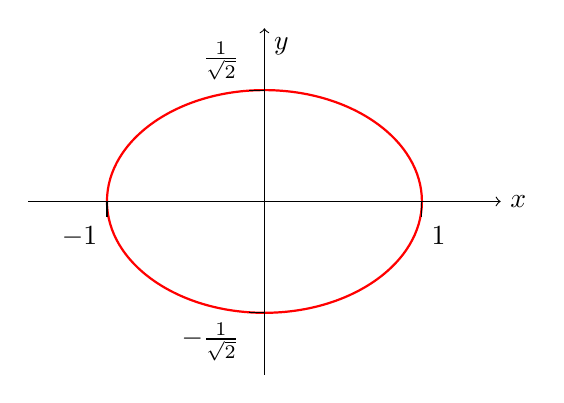
\begin{tikzpicture}[scale=2]
      \draw[thick,red,yscale={1/sqrt(2)}] (0,0) circle [radius=1];
      \draw[->] (-1.5,0) -- (1.5,0) node[right] {$x$};
      \draw[->] (0,-1.1) -- (0,1.1) node[below right] {$y$};
      \draw (-1,0) -- +(0,-.1) node[below left] {$-1$};
      \draw (1,0) -- +(0,-.1) node[below right] {$1$};
      \draw (0,{-1/sqrt(2)}) -- +(-.1,0) node[below left] {$-\frac{1}{\sqrt{2}}$};
      \draw (0,{1/sqrt(2)}) -- +(-.1,0) node[above left] {$\frac{1}{\sqrt{2}}$};
    \end{tikzpicture}
  \end{equation*}
\end{solution}

In general, for $a,b>0$, the curve $ax^2 + by^2 = 1$ is an ellipse
with $x$-intercepts $\pm 1/\sqrt{a}$ and $y$-intercepts
$\pm 1/\sqrt{b}$. Similarly, for $a,b,c>0$, the equation
$ax^2 + by^2 + cz^2 = 1$ describes a $3$-dimensional ellipsoid with
$x$-intercepts $\pm 1/\sqrt{a}$, $y$-intercepts $\pm 1/\sqrt{b}$, and
$z$-intercepts $\pm 1/\sqrt{c}$:
\begin{equation*}
  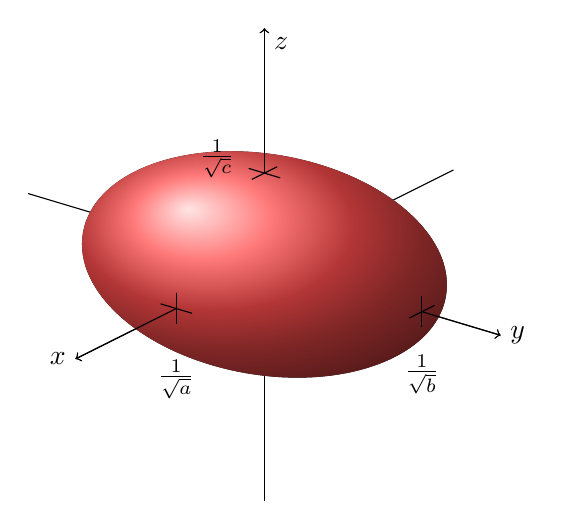
\begin{tikzpicture}[scale=2]
    \begin{scope}[y={(1cm,-0.3cm)},x={(-0.8cm,-0.4cm)},z={(0cm,1cm)}]
      \draw[->] (-1.5,0,0) -- (1.5,0,0) node[left] {$x$};
      \draw[->] (0,-1.5,0) -- (0,1.5,0) node[right] {$y$};
      \draw[->] (0,0,-1.5) -- (0,0,1.5) node[below right] {$z$};
    \end{scope}
    \fill[ball color=red!70] (0,0,0) circle [x radius=1.17, y radius=0.7, rotate=-10];
    \begin{scope}[y={(1cm,-0.3cm)},x={(-0.8cm,-0.4cm)},z={(0cm,1cm)}]
      \draw[->] (0.7,0,0) -- (1.5,0,0);
      \draw[->] (0,1,0) -- (0,1.5,0);
      \draw[->] (0,0,0.58) -- (0,0,1.5);
      \draw (0.7,0,0) -- +(0,0,0.1) -- +(0,0,-0.1) +(0,0,-0.45) node {$\frac{1}{\sqrt{a}}$};
      \draw (0.7,0,0) -- +(0,0.1,0) -- +(0,-0.1,0);
      \draw (0,1,0) -- +(0,0,0.1) -- +(0,0,-0.1) +(0,0,-0.4) node {$\frac{1}{\sqrt{b}}$};
      \draw (0,1,0) -- +(0.1,0,0) -- +(-0.1,0,0);
      \draw (0,0,0.58) -- +(-0.1,0,0) -- +(0.1,0,0);
      \draw (0,0,0.58) -- +(0,0.1,0) -- +(0,-0.1,0) +(0,-0.3,0) node {$\frac{1}{\sqrt{c}}$};
    \end{scope}
  \end{tikzpicture}
\end{equation*}

\noindent
Each ellipse or ellipsoid has a set of \textbf{principal axes}%
\index{principal axis}%
\index{quadratic form!principal axes}, which are its axes of
symmetry. When the quadratic forms are diagonal, as in the above
examples, the principal axes are the standard coordinate axes. When
the quadratic forms are not diagonal, the principal axes are the
eigenvectors of the matrix $A$. This is the content of the following
proposition.

\begin{proposition}{Principal axes of a quadratic form}{principal-axes}
  Consider a quadratic form in matrix form,
  $f(\vect{v}) = \vect{v}^TA\vect{v}$, where $A$ is a positive definite
  $n\times n$-matrix. Let $\set{\vect{u}_1,\ldots,\vect{u}_n}$ be an
  orthonormal set of eigenvectors of $A$, and let
  $\eigenvar_1,\ldots,\eigenvar_n$ be the corresponding eigenvalues.
  Then the solutions of the equation
  \begin{equation*}
    \vect{v}^TA\vect{v} = 1
  \end{equation*}
  form an $n$-dimensional ellipsoid whose principal axes are parallel
  to $\vect{u}_1,\ldots,\vect{u}_n$ and whose $\vect{u}_i$-intercepts
  are $\pm\frac{1}{\sqrt{\eigenvar_i}}$.  
\end{proposition}

\begin{proof}
  Let $P$ be the orthogonal matrix whose columns are
  $\vect{u}_1,\ldots,\vect{u}_n$. From the proof of
  Proposition~\ref{prop:quadratic-form-diagonalize}, we know that the
  equation $\vect{v}^TA\vect{v} = 1$ is equivalent to
  $\eigenvar_1y_1^2 + \ldots + \eigenvar_ny_n^2=1$, where
  $y_1,\ldots,y_n$ are variables such that
  \begin{equation}\label{eqn:principal-axes}
    \vect{v} = P\begin{mymatrix}{c} y_1 \\ \vdots \\ y_n \end{mymatrix}.
  \end{equation}
  Since $A$ is positive definite, we have
  $\eigenvar_1,\ldots,\eigenvar_n>0$ by
  Proposition~\ref{prop:characterize-positive}.  We therefore know
  that in the $(y_1,\ldots,y_n)$-coordinate system, the equation
  $\eigenvar_1y_1^2 + \ldots + \eigenvar_ny_n^2 = 1$ describes an
  ellipsoid whose $y_1$-intercepts are $\pm1/\sqrt{\eigenvar_1}$, whose
  $y_2$-intercepts are $\pm1/\sqrt{\eigenvar_2}$, and so on. The only
  thing that remains to do is to figure out the direction of the
  coordinate axes. The $y_1$-axis points in the direction of the point
  with coordinates $(y_1,\ldots,y_n) = (1,0,\ldots,0)$.  Using the
  change of variables formula {\eqref{eqn:principal-axes}}, we find
  that this corresponds to the first column of $P$, i.e.,
  $\vect{v}=\vect{u}_1$. Similarly, the $y_2$-axis points in the
  direction of $\vect{u}_2$, and so on.
\end{proof}

\begin{example}{Sketching a quadratic curve}{sketching-quadratic}
  Sketch the curve $3x^2 + 4xy + 6y^2 = 1$.
\end{example}

\begin{solution}
  The matrix for the quadratic form $3x^2 + 4xy + 6y^2$ is
  \begin{equation*}
    A = \begin{mymatrix}{rr} 3 & 2 \\ 2 & 6 \end{mymatrix}.
  \end{equation*}
  From Example~\ref{exa:quadratic-form-diagonalize}, we know that the
  normalized eigenvectors of $A$ are
  \begin{equation*}
    \vect{u}_1
    ~=~ \frac{1}{\sqrt{5}} \begin{mymatrix}{r} 1 \\ 2 \end{mymatrix}
    \quad\mbox{and}\quad
    \vect{u}_2
    ~=~ \frac{1}{\sqrt{5}} \begin{mymatrix}{r} -2 \\ 1 \end{mymatrix},
  \end{equation*}
  with respective eigenvalues $\eigenvar_1 = 7$ and $\eigenvar_2 =
  2$. Therefore, by Proposition~\ref{prop:principal-axes}, the curve
  $3x^2 + 4xy + 6y^2 = 1$ is an ellipse with principal axes
  $\vect{u}_1$ and $\vect{u}_2$, and with respective intercepts
  $\pm1/\sqrt{7}$ and $\pm1/\sqrt{2}$.
  \begin{equation*}
    \begin{tikzpicture}[scale=3]
      \begin{scope}[color=black]
        \draw[->] (-1.5,0) -- (1.5,0) node[right] {$x$};
        \draw[->] (0,-1.5) -- (0,1.5) node[below right] {$y$};
        \draw (-1,0) -- +(0,-.1) +(0,-0.2) node {$-1$};
        \draw (1,0) -- +(0,-.1) +(0,-0.2) node {$1$};
        \draw (0,-1) -- +(-.1,0) +(-0.2,0) node {$-1$};
        \draw (0,1) -- +(-.1,0) +(-0.2,0) node {$1$};
      \end{scope}
      \begin{scope}[color=blue,cm={(1/sqrt(5),2/sqrt(5),-2/sqrt(5),1/sqrt(5),(0,0))}]
        \draw[thick,red] (0,0) circle [x radius={1/sqrt(7)}, y radius={1/sqrt(2)}];
        \draw[->,blue!50] (-1.5,0) -- (1.5,0);
        \draw[->,blue!50] (0,-1.5) -- (0,1.5);
        \draw[blue!50] (-1,0) -- +(0,.1) +(0,0.2) node {$-1$};
        \draw[blue!50] (1,0) -- +(0,.1) +(0,0.2) node {$1$};
        \draw[blue!50] (0,-1) -- +(-.1,0) +(-0.2,0) node {$-1$};
        \draw[blue!50] (0,1) -- +(-.1,0) +(-0.2,0) node {$1$};
        \draw ({-1/sqrt(7)},0) -- +(0,.1) +(-0.15,0.2) node {$-\frac{1}{\sqrt{7}}$};
        \draw ({1/sqrt(7)},0) -- +(0,.1) +(0.1,0.15) node {$\frac{1}{\sqrt{7}}$};
        \draw (0,{-1/sqrt(2)}) -- +(-.1,0) +(-0.25,0) node {$-\frac{1}{\sqrt{2}}$};
        \draw (0,{1/sqrt(2)}) -- +(-.1,0) +(-0.225,0) node {$\frac{1}{\sqrt{2}}$};
        %\fill[color=black] (1,0) circle [radius=0.9pt] node[right=5pt] {$(x,y)=(\frac{1}{\sqrt{5}},\frac{2}{\sqrt{5}})$};
        %\fill[color=black] (0,1) circle [radius=0.9pt] node[left=11pt] {$(x,y)=(-\frac{2}{\sqrt{5}},\frac{1}{\sqrt{5}})$};
        \draw[thick,blue,->] (0,0) -- (1,0) node[right] {$\vect{u}_1$};
        \draw[thick,blue,->] (0,0) -- (0,1) node[above] {$\vect{u}_2$};
      \end{scope}
    \end{tikzpicture}
  \end{equation*}
\end{solution}

